\documentclass[journal,12pt,twocolumn]{IEEEtran}
\usepackage{tikz}
\usepackage{amsmath}
\usepackage{amssymb}
\pagestyle{empty}
\usepackage{setspace}
\singlespacing
\usepackage{caption}
\captionsetup{justification=centering}
\usepackage{amsthm}
\usepackage{mathtools} 
\usepackage{extarrows}
\usepackage{amssymb,amsmath}


\begin{document}
\newcommand{\myvec}[1]{\ensuremath{\begin{pmatrix}#1\end{pmatrix}}}
\newcommand{\cmyvec}[1]{\ensuremath{\begin{pmatrix*}[c]#1\end{pmatrix*}}}
\providecommand{\norm}[1]{\lVert#1\rVert}
\newcommand{\mydet}[1]{\ensuremath{\begin{vmatrix}#1\end{vmatrix}}}
\newcommand{\proj}[2]{\textbf{proj}_{\vec{#1}}\vec{#2}}
\newcommand{\abs}[1]{\left\lvert#1\right\rvert}
\newcommand{\RNum}[1]{\uppercase\expandafter{\romannumeral #1\relax}}
\newcommand{\Rnum}[1]{\lowercase\expandafter{\romannumeral #1\relax}}
\let\StandardTheFigure\thefigure
\let\vec\mathbf

\title{
BASICS OF PROGRAMMING

ASSIGNMENT - 2
}
\author{ LAKSHMI GAYATHRI GUDIPUDI - SM21MTECH11001}
\maketitle
\newpage
\bigskip
\renewcommand{\thefigure}{\theenumi}
\bibliographystyle{IEEEtran}
\section*{ Chapter \RNum{3} Ex-\RNum{4} Q-5}
\noindent
Find the condition that the lines
$$\mathbf{y+t_i x=2at_i+at_i^3}$$
where i=1,2,3, are concurrent. 
$$\mathbf{t_1 x + y = 2at_1 +at_1^3}$$
$$\mathbf{t_2 x + y = 2at_2 +at_2^3}$$
$$\mathbf{t_3 x + y = 2at_3 +at_3^3}$$
\noindent
\section*{\textbf{Solution}}
\noindent
Considering coefficients of three lines in matrix form :
\begin{align}
\myvec{t_1&1}\vec{x}=2at_1+at_1^3\\
\myvec{t_2&1}\vec{x}=2at_2+at_2^3\\
\myvec{t_3&1}\vec{x}=2at_3+at_3^3
\end{align}
The above equations form a matrix equation as below:
\begin{align}
\myvec{t_1&1\\t_2&1\\t_3&1}\vec{x}=\myvec{2at_1+at_1^3\\2at_2+at_2^3\\2at_3+at_3^3}
\end{align}
Given the lines are concurrent ,so considering above equations are  reduced to augmented form as below to find the condition for lines to be concurrent:
\begin{align}
\myvec{
t_1&1&2at_1+at_1^3\\
t_2&1&2at_2+at_2^3\\
t_3&1&2at_3+at_3^3
}
\end{align}

Performing row operations on the above augmented matrix as follows:

\begin{align}
\begin{split}
\myvec{
t_1&1&2at_1+at_1^3\\t_2&1&2at_2+at_2^3\\t_3&1&2at_3+at_3^3
}\\
R_2 \leftarrow {R_2-R_1}\\R_3 \leftarrow {R_3-R_1}\\
\myvec{t_1&1&t_1^3\\t_2-t_1&0&2at_2-2at_1+at_2^3-at_1^3\\t_3-t_1&0&2at_3-2at_1+at_3^3-at_1^3}\\
\myvec{t_1&1&t_1^3\\t_2-t_1&0&(t_2-t_1)(2a+a(t_2^2+t_1^2+t_1t_2))\\t_3-t_1&0&(t_3-t_1)(2a+a(t_3^2+t_1^2+t_3t_1))}\\
R_2 \leftarrow {R_2/(t_2-t_1)}\\R_3 \leftarrow {R_3/(t_3-t_1)}\\
(t_2-t_1)(t_3-t_1)\myvec{t_1&1&t_1^3\\1&0&2a+a(t_2^2+t_1^2+t_1t_2)\\1&0&2a+a(t_3^2+t_1^2+t_3t_1)}\\
R_3 \leftarrow {R_3-R_2)}\\
(t_2-t_1)(t_3-t_1)\myvec{t_1&1&t_1^3\\1&0&2a+a(t_2^2+t_1^2+t_1t_2)\\0&0&a(t_3^2-t_2^2+t_3t_1-t_1t_2)}\\
(t_2-t_1)(t_3-t_1)\myvec{t_1&1&t_1^3\\1&0&2a+a(t_2^2+t_1^2+t_1t_2)\\0&0&a(t_3-t_2)(t_2+t_1+t_3)}\\
R_3 \leftarrow {R_3/a(t_3-t_2)}\\
a(t_2-t_1)(t_3-t_1)(t_3-t_2)\myvec{t_1&1&t_1^3\\1&0&2a+a(t_2^2+t_1^2+t_1t_2)\\0&0&(t_2+t_1+t_3)}\\
\end{split}
\end{align}
Considering above matrix in echelon form the last row should be zero,so we get the condition for concurrency of lines as follows:
\begin{equation}
\begin{split}
(t_2-t_1)(t_3-t_1)(t_3-t_2)(t_2+t_3+t_1)=0
\end{split}
\end{equation}
\begin{equation}
(t_1-t_2)(t_2-t_3)(t_3-t_1)(t_1+t_2+t_3)=0
\label{eq:1}
\end{equation}

Therefore Equation \eqref{eq:1} represents the condition for the three lines to be concurrent.

Now considering lines as follows:
\begin{align}
\begin{split}
\mathbf{x + y = 3}\\
\mathbf{2x +y =12}\\
\mathbf{-3x+y =-33}
\end{split}
\end{align}
Now considering above lines in the format of lines given in question we get,
\begin{align}
\begin{split}
t_1=1\\
t_2=2\\
t_3=-3\\
\end{split}
\label{eq:2}
\end{align}
so from equation \eqref{eq:1} we got the condition ,so substituting values from equation \eqref{eq:2} in the condition we get:
\begin{align}
\begin{split}
(t_1-t_2)(t_2-t_3)(t_3-t_1)(t_1+t_2+t_3)=0\\
(1-2)(2-3)(-3-1)(1+2-3)=0
\end{split}
\end{align}
In the above equation LHS =RHS .Hence verified.

\begin{figure}[!ht]
    \centering
    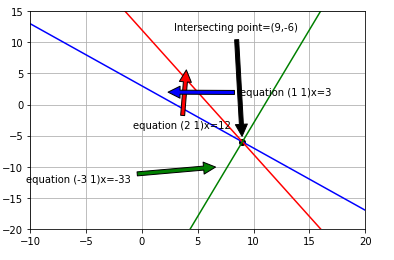
\includegraphics[width=\columnwidth]{assignment-2.PNG}
    \caption{Representation of lines intersecting at point(9,-6)}
    \label{fig:}
\end{figure}

\end{document}

